\documentclass[10pt,spanish]{article}  
\usepackage[spanish,es-nodecimaldot]{babel} %Indica que escribiermos en español y que no cambie los puntos y comas matematicos de ingles a español

\usepackage[utf8]{inputenc} %Indica qué codificación se está usando ISO-8859-1(latin1)  o utf8 
\selectlanguage{spanish}

%%%%%%% DEFINICIÓN DE VARIABLES %%%%%%%%%%%%%%%%%%%
\newcommand{\Practico}{Practico 1}
\newcommand{\Titulo}{Letra y Soluciones Oficiales del Kurose}
\newcommand{\Materia}{Redes de Computadoras}

%%%%%%%% PREÁMBULO %%%%%%%%%%%%

\usepackage{amsmath} % Comandos extras para matemáticas (cajas para ecuaciones,
% etc)
\usepackage{amssymb} % Simbolos matematicos (por lo tanto)
\usepackage{graphicx} % Incluir imágenes en LaTeX
\usepackage{color} % Para colorear texto
\usepackage{subfigure} % subfiguras
\usepackage{float} %Podemos usar el especificador [H] en las figuras para que se queden donde queramos
\usepackage{capt-of} % Permite usar etiquetas fuera de elementos flotantes
% (etiquetas de figuras)
\usepackage{sidecap} % Para poner el texto de las imágenes al lado
	\sidecaptionvpos{figure}{c} % Para que el texto se alinie al centro vertical
\usepackage{caption} % Para poder quitar numeracion de figuras
\usepackage{commath} % funcionalidades extras para diferenciales, integrales,
% etc (\od, \dif, etc)
\usepackage{cancel} % para cancelar expresiones (\cancelto{0}{x})


% MARGENES 
\usepackage{anysize} 					% Para personalizar el ancho de  los márgenes
\marginsize{2cm}{2cm}{2cm}{2cm} % Izquierda, derecha, arriba, abajo
\setlength{\parindent}{0cm}
\setlength{\parskip}{\baselineskip}

% Para que las referencias sean hipervínculos a las figuras o ecuaciones aparezcan en color
\usepackage[colorlinks=true,plainpages=true,citecolor=blue,linkcolor=blue]{hyperref}
%\usepackage{hyperref} 

% ENCABEZADO Y PIE DE PÁGINA
\usepackage{fancyhdr} 
\pagestyle{fancy}
\fancyhf{}

\fancyfoot[C]{\thepage}  % centro
\renewcommand{\footrulewidth}{0.4pt}

\usepackage[framemethod=tikz]{mdframed}
\newmdenv[
  topline=false, %oculta linea arriba
  bottomline=false, % oculta linea abajo
  rightline=false, % oculta linea derecha
  skipabove=\topsep,
  skipbelow=\topsep,
]{siderules}

\numberwithin{figure}{section} % numeración de figuras por seccion
\usepackage[font=bf,labelfont=bf]{caption} % setea estilo bf (bold) a los caption (texto y label)

\usepackage[compact]{titlesec} %Formato de las secciones
\titleformat*{\section}{\LARGE\bfseries}
\titleformat*{\subsection}{\Large\bfseries}
\titleformat*{\subsubsection}{\large\bfseries}


\usepackage{etoolbox} % Agrega puntos a las sections en el TOC
\makeatletter
\patchcmd{\l@section}
  {\hfil}
  {\leaders\hbox{\normalfont$\m@th\mkern \@dotsep mu\hbox{.}\mkern \@dotsep mu$}\hfill}
  {}{}
\makeatother

\usepackage{enumerate}% http://ctan.org/pkg/enumerate

\newcommand{\italic}[1]{\textit{#1}} % creo un alias del comando \textit para poner fuente italica

\setcounter{secnumdepth}{0} % evita que section haga numerado de secciones

\title{\Practico - \Titulo}

%%%%%%%% TERMINA PREÁMBULO %%%%%%%%%%%%

\begin{document}

%%%%%%%%%%%%%%%%%%%%%%%%%%%%%%%%%% PORTADA %%%%%%%%%%%%%%%%%%%%%%%%%%%%%%%%%%%%%%%%%%%%
%%%
\topskip0pt
\vspace*{\fill}
\begin{center}																		%%%
\newcommand{\HRule}{\rule{\linewidth}{0.5mm}}							
\textsc{\huge \Materia}\\[1.5cm]	

\textsc{\huge \Practico				%%%
}\\[1.5cm]													%%%
    																				%%%
\vspace*{5cm}																		%%%
																					%%%
\HRule \\[0.4cm]																	%%% 
{ \huge \bfseries \Titulo \\ \Large(Tomados de la $5^{ta}$ edición en inglés)}\\[0.3cm]	%%%
 																					%%%
\HRule \\[4cm]																	%%%
%%%
																		
\end{center}							 								\vspace*{\fill}		
																					
%%%%%%%%%%%%%%%%%%%% TERMINA PORTADA %%%%%%%%%%%%%%%%%%%%%%%%%%%%%%%%
\newpage
\tableofcontents

\newpage
\section[Problema 1]{Problema 1 \textnormal{\Large{(Ref. Cap. 1 Prob. 2)}}}
Consider an application that transmits data at a steady rate (for example, the sender generates an $N$-bit unit of data every $k$ time units, where $k$ is small and fixed). Also, when such an application starts, it will continue running for a relatively long period of time. Answer the following questions, briefly justifying your answer:

\renewcommand{\theenumi}{\alph{enumi}} % Cambia la numeracion a letras
\begin{enumerate}
\item Would a packet-switched network or a circuit-switched network be more appropriate for this application? Why?
\item Suppose that a packet-switched network is used and the only traffic in this network comes from such applications as described above. Furthermore, assume that the sum of the application data rates is less than the capacities of each and every link. Is some form of congestion control needed? Why?
\end{enumerate}

\subsection*{Respuesta}

\begin{enumerate}
\item A circuit-switched network would be well suited to the application described, because the application involves long sessions with predictable smooth bandwidth requirements. Since the transmission rate is known and not bursty, bandwidth can be reserved for each application session circuit with no significant waste. In addition, we need not worry greatly about the overhead costs of setting up and tearing down a circuit connection, which are amortized over the lengthy duration of a typical application session.

\item Given such generous link capacities, the network needs no congestion control mechanism. In the worst (most potentially congested) case, all the applications simultaneously transmit over one or more particular network links. However, since each link offers sufficient bandwidth to handle the sum of all of the applications' data rates, no congestion (very little queuing) will occur.
\end{enumerate}

\section[Problema 2]{Problema 2 \textnormal{\Large{(Ref. Cap. 1 Prob. 5)}}}
This elementary problem begins to explore propagation delay and transmission delay, two central concepts in data networking. Consider two hosts, A and B, connected by a single link of rate $R$ bps. Suppose that the two hosts are separated by $m$ meters, and suppose the propagation speed along the link is $s$ meters/sec. Host A is to send a packet of size $L$ bits to Host B.
\begin{enumerate}
\item Express the propagation delay, $d_{prop}$  in terms of $m$ and $s$.
\item Determine the transmission time of the packet, $d_{trans}$, in terms of $L$ and $R$.
\item Ignoring processing and queuing delays, obtain an expression for the end- to-end delay.
\item Suppose Host A begins to transmit the packet at time $t = 0$. At time $t = d_{trans}$, where is the last bit of the packet?
\item Suppose $d_{prop}$ is greater than $d_{trans}$. At time $ t= d_{trans}$, where is the first bit of the packet?
\item Suppose $d_{prop}$ is less than $d_{trans}$. At time $t = d_{trans}$, where is the first bit of the packet?
\item Suppose $s = 2.5 \cdot 10^8$, $L$ = 120 bits, and $R$=56 kbps. Find the distance $m$ so that $d_{prop}$ equals $d_{trans}$.
\end{enumerate}

\subsection*{Respuesta}

\begin{enumerate}
\item $d_{prop}$ = $\displaystyle \frac{m}{s}$ seconds.
\item $d_{trans}$ = $\displaystyle \frac{L}{R}$ seconds.
\item $\displaystyle d_{end-to-end} = \left( \frac{m}{s} + \frac{L}{R} \right)$ seconds.
\item The bit is just leaving Host A.
\item The first bit is in the link and has not reached Host B.
\item The first bit has reached Host B.
\item Want $\displaystyle m = \frac{L}{R} s = \frac{120}{56 \times 10^3} (2.5 \times 10^8) = 536 km$
\end{enumerate}

\section[Problema 3]{Problema 3 \textnormal{\Large{(Ref. Cap. 1 Prob. 9)}}}
Consider a packet of length $L$ which begins at end system A and travels over three links to a destination end system. These three links are connected by two packet switches. Let $d_i$, $s_i$, and $R_i$ denote the length, propagation speed, and the transmission rate of link $i$, for $i$ = 1, 2, 3. The packet switch delays each packet by $d_{proc}$. Assuming no queuing delays, in terms of $d_i$, $s_i$, $R_i$, ($i$ = 1,2,3), and $L$, what is the total end-to-end delay for the packet? Suppose now the packet is 1,500 bytes, the propagation speed on both links is $2.5 \cdot 10^8$ m/s, the transmission rates of all three links are 2 Mbps, the packet switch processing delay is 3 msec, the length of the first link is 5,000 km, the length of the second link is 4,000 km, and the length of the last link is 1,000 km. For these values, what is the end-to-end delay?

\subsection*{Respuesta}

The first end system requires $L/R_1$ to transmit the packet onto the first link; the packet propagates over the first link in $d_1 / s_1$; the packet switch adds a processing delay of $d_{proc}$; after receiving the entire packet, the packet switch connecting the first and the second link requires $L / R_2$ to transmit the packet onto the second link; the packet propagates over the second link in $d_2 / s_2$. Similarly, we can find the delay caused by the second switch and the third link: $L / R_3$, $d_{proc}$, and $d_3 / s_3$.\\
Adding these five delays gives: $d_{end-end} = (L / R_1) + (L / R_2) + (L / R_3) + (d_1 / s_1) + (d_2 / s_2) + (d_3 / s_3) + d_{proc} + d_{proc}$\\
 \\
To answer the second question, we simply plug the values into the equation to get 6 + 6 + 6 + 20+16 + 4 + 3 + 3 = 64 msec.

\section[Problema 4]{Problema 4 \textnormal{\Large{(Ref. Cap. 1 Prob. 10)}}}

In the above problem, suppose $R_1 = R_2 = R_3 = R$ and $d_{proc}$ = 0. Further suppose the packet switch does not store-and-forward packets but instead immediately transmits each bit it receives before waiting for the packet to arrive. What is the end-to-end delay?

\subsection*{Respuesta}

Because bits are immediately transmitted, the packet switch does not introduce any delay; in particular, it does not introduce a transmission delay. Thus,\\
 \\
$d_{end-end} = (L / R) + (d_1 / s_1) + (d_2 / s_2) + (d_3 / s_3)$
                    
For the values in Problem 9, we get 6 + 20 + 16 + 4 = 46 msec.


\section[Problema 5]{Problema 5 \textnormal{\Large{(Ref. Cap. 1 Prob. 12)}}}

Suppose $N$ packets arrive simultaneously to a link at which no packets are currently being transmitted or queued. Each packet is of length $L$ and the link has transmission rate $R$. What is the average queuing delay for the $N$ packets?

\subsection*{Respuesta}

The queuing delay is 0 for the first transmitted packet, $L/R$ for the second transmitted packet, and generally, $(n-1)(L/R)$ for the $n^{th}$ transmitted packet. Thus, the average delay for the N packets is\\
 \\
$(L/R + 2L/R + ....... + (N-1)L/R)/N\\ 
= L/(RN) * (1 + 2 + ..... + (N-1))\\ 
= L/(RN) * N(N-1)/2\\
= LN(N-1)/(2RN)\\              
= (N-1)L/(2R)\\
$\\     
Note that here we used the well-known fact that $1 + 2 + ....... + N = N(N+1)/2$

\section[Problema 6]{Problema 6 \textnormal{\Large{(Ref. Cap. 1 Prob. 17)}}}

\begin{enumerate}
\item Generalize the end-to-end delay formula in Section 1.4.3 for heterogeneous processing rates, transmission rates, and propagation delays.
[Nota: La fórmula dada en la Sección 1.4.3 de la 5ta. Edición del Kurose  es, para el caso de retardo medio de cola despreciable, $d_{terminal-terminal} = N \cdot (d_{proc} + d_{trans} + d_{prop})$]
\item Repeat (a), but now also suppose that there is an average queuing delay of $d_{queue}$ at each node.
\end{enumerate}

\subsection*{Respuesta}
\begin{enumerate}
\item There are $Q$ nodes (the source host and the $Q-1$ routers). Let $d_{proc}^{q}$ denote the processing delay at the $q$ th node. Let $R^q$ be the transmission rate of the $q$ th link and let $d^q_{trans} = L/R^q$ .Let $d_{prop}^q$ be the propagation delay across the $q$ th link. Then
\begin{align*}
\displaystyle d_{end-to-end} = \sum^Q_{q=1} \left[ d^q_{proc} + d^q_{trans} + d^q_{prop} \right]
\end{align*}
\item Let $d^q_{queue}$ denote the average queuing delay at node $q$. Then
\begin{align*}
\displaystyle d_{end-to-end} = \sum^Q_{q=1} \left[ d^q_{proc} + d^q_{trans} + d^q_{prop} + d^q_{queue} \right]
\end{align*}

\end{enumerate}

\section[Problema 7]{Problema 7 \textnormal{\Large{(Ref. Cap. 1 Prob. 22)}}}

Consider Figure 1.19(a). Assume that we know the bottleneck link along the path from the server to the client is the first link with rate $R_s$ bits/sec. Suppose we send a pair of packets back to back from the server to the client, and there is no other traffic on this path. Assume each packet of size $L$ bits, and both links have the same propagation delay $d_{prop}$.

\begin{enumerate}
\item What is the packet inter-arrival time at the destination? That is, how much time elapses from when the last bit of the first packet arrives until the last bit of the second packet arrives?
\item Now assume that the second link is the bottleneck link (i.e., $R_c < R_s$). Is it possible that the second packet queues at the input queue of the second link? Explain. Now suppose that the server sends the second packet $T$ seconds after sending the first packet. How large must $T$ be to ensure no queuing before the second link? Explain.
\end{enumerate}
\begin{figure}[H]
\centering
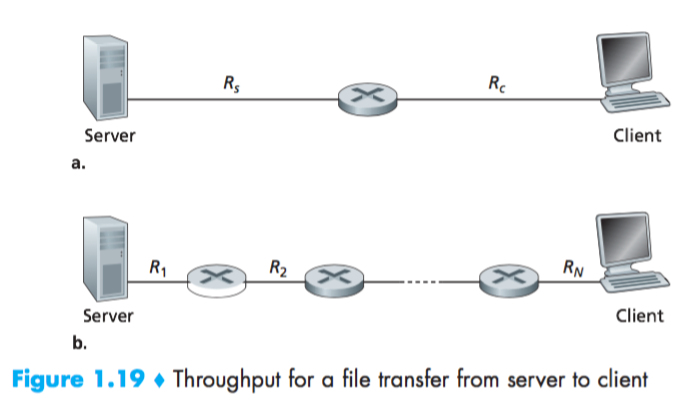
\includegraphics[width=0.7\textwidth]{Practico1/Fig1-19.png}
\end{figure}

\subsection*{Respuesta}

Lets call the first packet A and call the second packet B.
\begin{enumerate}
\item If the bottleneck link is the first link, then, packet B is queued at the first link waiting for the transmission of packet A. So, the packet inter-arrival time at the destination is simply $L/R_s$.
\item If the second link is the bottleneck link and since both packets are sent back to back, it must be true that the second packet arrives at the input queue of the second link before the second link finishes the transmission of the first packet. That is,
\begin{equation} L/R_s + L/R_s + d_{prop} < L/Rs + dprop + L/Rc \end{equation}
The left hand side of the above inequality represents the time needed by the second packet to \italic{arrive at} the input queue of the second link (the second link has not started transmitting the second packet yet).\\
The right hand side represents the time needed by the first packet to finish its transmission onto the second link.\\
 \\
We know that (1) is possible as $R_c < R_s$. And it is clear that (1) shows that the second packet must have queuing delay at the input queue of the second link.\\
If we send the second packet $T$ seconds later, then we can ensure the there is no queuing delay for the second packet at the second link if we have,\\
$L/R_s + L/R_s + d_{prop} + T >= L/R_s + d_{prop} + L/R_c$\\
Thus, $T$ must be $L/R_c - L/R_s$.
\end{enumerate}

\section[Problema 8]{Problema 8 \textnormal{\Large{(Ref. Cap. 1 Prob. 24)}}}

Suppose two hosts, A and B, are separated by 20,000 kilometers and are connected by a direct link of $R$ = 2 Mbps. Suppose the propagation speed over the link is $2.5 \cdot 10^8$ meters/sec.
\begin{enumerate}
\item Calculate the bandwidth-delay product, $R \cdot d_{prop}$.
\item Consider sending a file of 800,000 bits from Host A to Host B. Suppose the file is sent continuously as one large message. What is the maximum number of bits that will be in the link at any given time?
\item Provide an interpretation of the bandwidth-delay product.
\item What is the width (in meters)of a bit in the link? Is it longer than a fooball field?
\item Derive a general expression for the width of a bit in terms of the propagation speed $s$, the transmission rate $R$, and the length of the link $m$.

\end{enumerate}

\subsection*{Respuesta}

\begin{enumerate}
\item 160,000 bits
\item 160,000 bits
\item The bandwidth-delay product of a link is the maximum number of bits that can be in the link.
\item the width of a bit = length of link / bandwidth-delay product, so 1 bit is 125 meters long, which is longer than a football field.
\item $s/R$

\end{enumerate}

\section[Problema 9]{Problema 9 \textnormal{\Large{(Ref. Cap. 1 Prob. 25)}}}

Referring to problem P24 (\textbf{Problema 8 del Práctico}), suppose we can modify R. For what value of R is the width of a bit as long as the length of the link?

\subsection*{Respuesta}

$\displaystyle \frac{s}{R} = 20000km \text{, then } R = \frac{s}{20000km} = \frac{2.5 \cdot 10^8}{2 \cdot 10^7}= 12.5 bps$

\section[Problema 10]{Problema 10 \textnormal{\Large{(Ref. Cap. 1 Prob. 26)}}}

Consider problem P24 (\textbf{Problema 8 del Práctico}) but now with a link of $R$ = 1 Gbps.
\begin{enumerate}
\item Calculate the bandwidth-delay product, $R \cdot d_{prop}$.
\item Consider sending a file of 800,000 bits from Host A to Host B. Suppose the file is sent continuously as one big message. What is the maximum number of bits that will be in the link at any given time?
\item What is the width (in meters) of a bit in the link?
\end{enumerate}

\subsection*{Respuesta}

\begin{enumerate}
\item 80,000,000 bits
\item 800,000 bits, this is because that the maximum number of bits that will be in the link at any given time = $min(\text{bandwidth delay product}, \text{packet size})$ = 800,000 bits.
\item .25 meters
\end{enumerate}

\section[Problema 11]{Problema 11 \textnormal{\Large{(Ref. Cap. 1 Prob. 28)}}}

Suppose there is a1 0Mbps microwave link between a geostationary satellite and its base station on Earth. Every minute the satellite takes a digital photo and sends it to the base station. Assume a propagation speed of $2.4 \cdot 10^8$ meters/sec.

\begin{enumerate}
\item What is the propagation delay of the link?
\item What is the bandwidth-delay product, $R \cdot d_{prop}$?
\item Let $x$ denote the size of the photo. What is the minimum value of $x$ for the microwave link to be continuously transmitting?
\end{enumerate}

\subsection*{Respuesta}

Recall geostationary satellite is 36,000 kilometers away from earth surface.
\begin{enumerate}
\item 150 msec
\item 1,500,000 bits
\item 600,000,000 bits
\end{enumerate}

\newpage

\section[Problema 12]{Problema 12 \textnormal{\Large{(Ref. Cap. 1 Prob. 30)}}}

In modern packet-switched networks, the source host segments long, application-layer messages (for example, an image or a music file) into smaller packets and sends the packets into the network. The receiver then reassembles the packets back into the original message. We refer to this process as \italic{message segmentation}. Figure 1.28 illustrates the end-to-end transport of a message with and without message segmentation. Consider a message that is $8 \cdot 10^6$ bits long that is to be sent from source to destination in Figure 1.28. Suppose each link in the figure is 2 Mbps. Ignore propagation, queuing, and processing delays.

\begin{figure}[H]
\centering
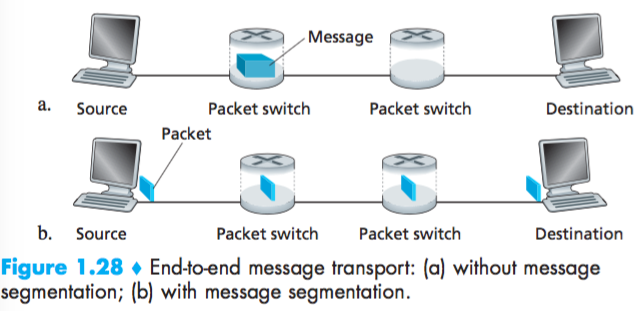
\includegraphics[width=0.7\textwidth]{Practico1/Fig1-28.png}
\end{figure}

\begin{enumerate}
\item Consider sending the message from source to destination $without$ message segmentation. How long does it take to move the message from the source host to the first packet switch? Keeping in mind that each switch uses store-and-forward packet switching, what is the total time to move the message from source host to destination host?
\item Now suppose that the message is segmented into 4,000packets, with each packet being 2,000 bits long. How long does it take to move the first packet from source host to the first switch? When the first packet is being sent from the first switch to the second switch, the second packet is being sent from the source host to the first switch. At what time will the second packet be fully received at the first switch?
\item How long does it take to move the file from source host to destination host when message segmentation is used? Compare this result with your answer in part (a) and comment.
d. Discuss the drawbacks of message segmentation.
\end{enumerate}

\subsection*{Respuesta}

\begin{enumerate}
\item Time to send message from source host to first packet switch =\\
$\displaystyle \frac{8 \times 10^6}{2 \times 10^6}$ sec = 4sec. With store-and-forward switching, the total time to move message from source host to destination host = 4 sec $\times$ 3 hops = 12 sec
\item Time to send $1^{st}$ packet from source host. to first packet switch =\\
$\displaystyle \frac{2 \times 10^3}{2 \times 10^6}$ sec = 1msec. Time at which $2^{nd}$ packet is received at the first switch = time at which 1st packet is received at the second switch = 2 $\times$ 1 msec = 2 msec.
\item Time at which 1st packet is received at the destination host =\\
1 m sec $\times$ 3 hops = 3 msec . After this, every 1 msec one packet will be received; thus time at which last ($4000^{th}$) packet is received =\\
3 msec + 3999 $\cdot$ 1m sec = 4.002 sec . It can be seen that delay in using message segmentation is significantly less (almost $1/3^{rd}$).
\item Drawbacks:
\begin{enumerate}
\item[i.] Packets have to be put in sequence at the destination.
\item[ii.] Message segmentation results in many smaller packets. Since header size is usually the same for all packets regardless of their size, with message segmentation the total amount of header bytes is more.
\end{enumerate}
\end{enumerate}
\end{document}
